% ch-firstrun.tex -- the first calculation, start to finish
\chapter{最初の計算}
\label{ch:firstrun}

本章では、一つのケースを最初から最後まで実行して出力を確認し、
設定を一つずつ変えてみる。入力ファイルのどこが結果のどこに効くかを
つかむのが目的である。Yuzenは\cref{ch:installation}の手順でビルド済みとする。

\section{ケースの実行}
\label{sec:firstrun:run}

実行時に与える引数は入力ファイル一つだけである。

\begin{shell}
cd <repository root>
mkdir -p run1 && cd run1
../build/bin/yuzen ../cases/tutorial_1d.toml
\end{shell}

入力ファイルのパスは相対でも絶対でもよく、空白や非ASCII文字を含んでいてもよい。
入力ファイルのほかに指定できるオプションは三つある。
\code{--check-input FILE}はファイルを読み込んで検査するだけで、計算は行わない
（\cref{sec:inputformat:unknown}）。\code{--help}は使い方を、
\code{--version}はバージョンを表示する。引数がない、入力ファイルが二つある、
未知のオプションがあるなど、これ以外の場合は使い方を標準エラー出力に表示し、終了コード1で終了する。
入力ファイルが存在しない場合、ディレクトリである場合、読み込めない場合も同じである。
終了コードの一覧は\cref{tab:exitcodes}に示す。

起動すると、バナー、バージョン、OpenMPのスレッド数を表示する。続いて入力を読み込んで整合性を検査し、
結果ディレクトリを作成して時間進行を始める。結果ディレクトリの名前は入力ファイル名ではなく、
入力ファイル中の\key{JobName}キーで決まる。この実行では
\file{tutorial\_1d/}が作られる。\file{cases/}以下のケースはどれも\key{JobName}に
自身のファイル名を設定しているので、結果ディレクトリ名は元のケース名と同じになる。

\begin{note}[作業用ディレクトリで実行する]
  出力は作業ディレクトリを基準に書き出されるので、結果を置きたい場所で実行する。
  \file{tools/run\_case.sh}はこの処理に加えて、スレッド数の固定とログの保存も行う
  （\cref{sec:env:tools}）。
  \begin{shell}
./tools/run_case.sh cases/leveling_1d_reg.toml runs/reg 1
  \end{shell}
\end{note}

ここで用いる\file{cases/tutorial\_1d.toml}は、1-Dの鉛直一様モデルの液膜である。
幅\SI{1}{\milli\metre}、セル数\SI{300}{}、膜厚スケール\SI{10}{\micro\metre}とし、
毛管レベリング、マランゴニ応力、蒸発を有効にして\SI{0.5}{\second}まで計算する。
計算は数秒で終わる。

\section{出力ファイル}
\label{sec:firstrun:output}

\begin{plain}
tutorial_1d/
  tutorial_1d.toml        a copy of the input, so the directory is self-describing
  JobInfo.txt             version, machine, linear-solver backends, start and end time
  Warnings.txt            warnings; zero-length if there were none
  FatalErrors.txt         why the run aborted; zero-length if it did not
  field00000.dat ...      the field, as tab-separated text (also the restart format)
  field00000.vts ...      the same field as VTK structured grid
  field00000.state ...    what a restart needs beyond the field (time, step, totals)
  tutorial_1d.pvd         ParaView time series pointing at the .vts files
  History.dat             volume, mean concentration, extrema, conservation error
  CalcInfo.dat            per-output-interval solver diagnostics
\end{plain}

まず端末の表示を確認し、次に一覧の上のほうにあるテキストファイルを参照されたい。

\paragraph{端末}には実行ログが表示される。ログは標準出力に出るだけで、結果ディレクトリには
保存されない。表示の冒頭には、ソルバーが入力から組み立てた設定が並ぶ。
各方程式の線形ソルバーのバックエンドと対流スキーム、格子、無次元化に用いたスケール
（\code{Scaling factors}の下の$L_0$、$H_0$、$T_0$、$U_0$）とそこから求めた無次元数、
モデルである。その後は進行状況のログになる。
ドット一つが1時間刻みに対応し、\code{dt+}と\code{dt-}は適応時間刻みによる刻みの増加と減少、
\code{Field file $n$, Time = $\dots$}は場の書き出しを表す。実行の最後には終了メッセージが
表示される。最初に確認すべきはこのメッセージである。

\begin{plain}
############## Time reached to the EndTime. #############
Field file 5, Time = 1.606806e-05
Largest Courant number of Numerics.Convection.Height = "Koren": 0.000469

############## Program normally terminated. #############
\end{plain}

正常終了には\code{Time reached to the EndTime.}、
\code{Dry out.}、\code{Steady state.}の三種類があり、ケースにとっての意味はかなり異なる。
それぞれの意味は\cref{sec:convergence:termination}で説明する。十数ステップで
\code{Steady state.}と報告された場合、多くは物理ではなく判定基準の問題を
示している。その理由も同じ節で述べる。

ログを残すには、自分でリダイレクトする（\code{yuzen case.toml > run.log}）か、
\file{tools/run\_case.sh}を用いる。後者はリダイレクトを代わりに行い、端末に表示される
内容をすべて実行ディレクトリの\file{stdout.txt}に保存する。

実行を途中で止めるには、Ctrl-Cを一度押す。計算中のステップを終えてから、その時点の状態を場ファイルと
\file{.state}に書き出し、\code{Program stopped by SIGINT; its output is complete.}
と表示して終了する。このファイルからリスタートでき（\cref{sec:firstrun:restart}）、
続きの計算結果は中断しなかった場合とビット単位で一致する。Ctrl-Cを二度押すと、プロセスは
直ちに終了する。詳細とディスクが満杯になった場合の挙動は\cref{sec:output:failures}に示す。

\paragraph{\file{JobInfo.txt}}には、バージョン、コンパイラ、マシン、開始・終了時刻と、
入力から決まる一つのセクションが記録される。このセクションには、モデルと、各方程式で実際に用いた線形ソルバーの
バックエンドが書かれる（\cref{sec:output:jobinfo}）。結果が桁違いにおかしく見えるときに
確認すべきスケール（$L_0$、$T_0$、$U_0$）は、ここではなく実行ログにある
（\cref{sec:governing:scales}）。

\paragraph{\file{Warnings.txt}}は必ず作成され、バナーは書かれない。そのため
\textbf{長さがゼロになるのは警告が一つも出なかった場合であり、その場合に限られる}。何か書かれていれば、
それは本物の警告である。

\paragraph{\file{FatalErrors.txt}}も必ず作成され、実行が異常終了しない限り長さはゼロである。
異常終了した場合は、その理由がこのファイル\emph{と}標準エラー出力の両方に書かれる。
メッセージは結果ディレクトリと端末の両方に残る。読むべきファイルがないのは、
ソルバーが入力を受け付けなかった場合だけである。このときは結果ディレクトリが作られる前に終了するので、
メッセージは標準エラー出力にしか出ない（\cref{sec:output:warnings}）。

\section{場ファイルの読み方}
\label{sec:firstrun:fields}

\file{field00000.dat}は、1行のヘッダーをもつタブ区切りのテキストである。1-Dの場合は次のようになる。

\begin{plain}
xx[mm]  HS[um]  Ux[m/s]  CC[-]  HH[um]  SS[um]
-5.00000000000000111e-01  5.00000000000000000e+00  0.0 ...
\end{plain}

\begin{yzntable}{\file{field*.dat}の列\label{tab:fieldcols}}{@{}L{0.09\textwidth} L{0.13\textwidth} L{0.70\textwidth}@{}}
\textsf{\bfseries 1-D} & \textsf{\bfseries 2-D} & \textsf{\bfseries 意味}\\ \midrule
\code{xx} & \code{xx}, \code{yy} & 面内座標（\si{\milli\metre}） \\
\code{HS} & \code{HS}            & 自由表面の高さ$h + s$（\si{\micro\metre}） \\
\code{Ux} & \code{Ux}, \code{Uy} & 面内速度。有効な項をすべて合わせた速度（\si{\metre\per\second}） \\
\code{CC} & \code{CC}            & 溶質濃度（質量分率） \\
\code{HH} & \code{HH}            & 膜厚$h$（\si{\micro\metre}） \\
\code{SS} & \code{SS}            & 基板の高さ$s$（\si{\micro\metre}） \\
\end{yzntable}

表の単位は、\key{Output.Dimensioned}が既定値の\val{true}の場合である。
\val{false}にすると、すべての列が無次元になる。面内方向と面外方向で長さの単位が\emph{異なる}
点に注意する。上の例の行で、中心から\SI{0.5}{\milli\metre}の点が$-0.5$、厚さ
\SI{5}{\micro\metre}の液膜が$5.0$となっているのはこのためである。

\begin{warn}[\code{HS}は自由表面、\code{HH}は膜厚]
  二列目は$h$ではなく$h+s$である。各列の関係を\cref{fig:film-geometry}に示す。
  濃度は最後の列ではなく四列目にある。
\end{warn}

\begin{figure}[tbp]
  \centering
  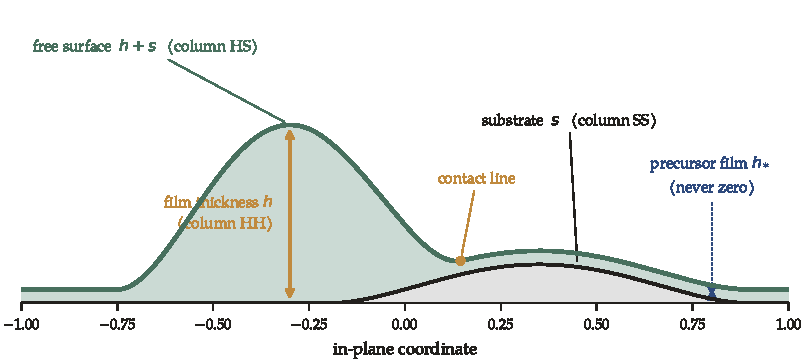
\includegraphics[width=\textwidth]{figures/film-geometry.pdf}
  \caption{\file{field*.dat}にある三つの高さの列。凹凸のある基板の上で、前駆膜に載った液滴を例に示す。
    \code{SS}は基板$s$、\code{HS}は目に見える形状である自由表面$h+s$、
    \code{HH}はその差である膜厚$h$である。平坦な基板では\code{HS}と\code{HH}が一致するため、
    区別は見えない。基板形状がある場合、両者の違いは、目に見える表面と実際にある液の層の違いになる。
    \key{Initial.\bk SurfaceShape.\bk PrecursorRatio}で設定する前駆膜$h_*$は
    \code{HH}の下限である。したがって接触線は膜厚がゼロになる点ではなく、
    自由表面が前駆膜に接する位置である（\cref{ch:wetting}）。
    \label{fig:film-geometry}}
\end{figure}

値が有次元か無次元かは\key{Output.Dimensioned}で決まる。どちらの場合も、値は
有効数字18桁で書き出される。このファイルがASCII形式のリスタートファイルを兼ねるためである。
既定の六桁では、膜厚の二階差分をとる（$\Delta x^2$で割る）ときに圧力が正しく求まらない。
$\Delta x = \SI{0.3}{\micro\metre}$の接触線用の格子では、出力精度だけが原因で圧力が数パーセント、
そこから求めた速度が三桁ずれた。

形状をざっと見るだけなら、どの描画ツールを使ってもよい。

\begin{shell}
gnuplot -p -e 'plot "tutorial_1d/field00004.dat" u 1:2 w l title "free surface"'
\end{shell}

\section{ParaViewでの表示}
\label{sec:firstrun:paraview}

\file{tutorial\_1d/tutorial\_1d.pvd}を開く。このファイルは各\file{.vts}ファイルとその時刻をまとめた
コレクションなので、ParaViewは時系列全体を正しい時刻とともに一度に読み込める。
連番ファイルのように、ParaViewに時刻を推測させる必要はない。VTKファイルが不要なら
\key{Output.FieldData.VTKFile}を\val{false}にする。テキストファイルの出力は
\key{NeutralFile}で別に制御する。

\section{設定を一つずつ変える}
\label{sec:firstrun:changing}

ケースをコピーして編集する。以下の変更は、おおむね最初に試すべき順に並べてある。

\paragraph{計算時間を変える。} \key{Numerics.EndTime}で指定し、単位は秒である。
既定値は\val{0}である。これは「制限なし」ではなく、1ステップで実行を止めるという意味なので、
必ず設定する。

\paragraph{出力の頻度を上げる。} 場は\key{Output.\bk FieldData.\bk TimeInterval}、
スカラーの履歴は\key{Output.\bk GeneralHistory.\bk TimeInterval}、
ソルバーの診断情報は\key{Output.\bk CalcInfo.\bk TimeInterval}で制御し、三つは互いに独立である。
履歴と診断情報は出力の負荷が小さいので、場の十倍から百倍の頻度で書くのが普通である。

\paragraph{格子を細かくする。} \key{Grid.Nx}で指定し、内部セルだけを数える。
格子を細かくすると、思わぬ代償がある。ニュートン修正量はある下限より小さくならない。
その下限のうち、行列要素との積として作られる項に由来する部分は、時間刻みとともに、
また格子が細かいほど大きくなる（\cref{sec:convergence:floor}）。格子を細かくしたケースが急に非常に遅くなったら、
ほかの設定を変える前に\cref{sec:convergence:absolute}を参照されたい。

\paragraph{物理項を有効・無効にする。} \key{Physics}以下の各項には\key{Enable}がある。
\file{tutorial\bk\_1d.toml}では鉛直重力、面内重力、遠心力、ソース項を無効にしている。
これらをすべて有効にした同じケースが\file{cases/\bk allphys\_1d\_reg.toml}である。

\paragraph{乾燥させる。} \key{Physics.Evaporation.Coef}は蒸発速度で、単位は
\si{\metre\per\second}である。この値は$\Ev$と$\Pen$の両方に入る。溶媒が抜けるにつれて
\file{History.dat}の\code{AveC}が上がっていく様子が確認できる。このケースのように粘度の指数が10の
場合、濃度が0.1変わると粘度は$e$倍になり、液膜は目に見えて流れなくなる。この連成は
ソルバーの中で最も強い非線形性である（\cref{sec:conc:properties}）。

\paragraph{接触線を加える。} \key{Physics.DisjoiningPressure}を有効にし、
\key{ContactAngle}、\key{ExponentN}、\key{ExponentM}、
\key{Initial.SurfaceShape.PrecursorRatio}を設定する。その前に必ず
\cref{sec:wetting:sizing}を参照されたい。接触角を指定すると、格子と液滴の高さを自由に
選べなくなる。二つの寸法規則を守らないケースは、もっともらしく見えるが角度の誤った
解を出す。

\section{リスタート}
\label{sec:firstrun:restart}

\file{field*.dat}はリスタート形式を兼ねているので、どの出力からでも計算を再開できる。
\key{Restart}を有効にし、ファイルを指定する。

\begin{toml}
[Restart]
Enable      = true
ASCII       = true
FileName    = "tutorial_1d/field00005.dat"
RestartTime = 0.501237
FileIndex   = 6
\end{toml}

あわせて、絶対時刻で指定する\key{Numerics.EndTime}を\key{RestartTime}より大きくする。
\key{RestartTime}には、\file{tutorial\_1d.pvd}に記載されたそのファイルの時刻を書く。場は
予定時刻ちょうどではなく、予定時刻に最も近いステップで書き出されるからである。この時刻を与えると、
場ファイルと同じ場所にある\file{field00005.state}も読み込み、中断しなかった場合とまったく同じように
計算を続ける（\cref{sec:ref-numerics:restart}）。このとき実行ログには
\code{continuing exactly from tutorial\_1d/field00005.state}と表示される。異なる時刻を
与えた場合は場だけを読み込み、その旨を表示する。

\key{FileName}は、結果ディレクトリではなく\textbf{ソルバーを起動した作業ディレクトリ}を基準とする
相対パスである。上の実行のファイルは\file{tutorial\_1d/}に書き出されたので、
同じディレクトリから実行するにはパスにこの接頭辞が必要である。\file{field00005.dat}だけで
済むのは\file{tutorial\_1d/}の中で実行した場合に限られるが、その場合は新しい実行も
同じ場所に結果を書き出そうとする。

リスタートでは、\key{Initial.SurfaceShape}の形状は読み込まれるが使われない。解析的に作った初期状態を
与えるときもこの方法を使う。\file{cases/eq/}と\file{cases/wet\_*.toml}のケースは、
\file{tools/make\_equilibrium\_1d.py}で作った平衡液滴から計算を始める。
接触線に見せかけの速度が生じた状態で計算が始まるのを避けるためである。キーは
\cref{ch:ref-numerics}に、平衡液滴の作り方は\cref{sec:wetting:equilibrium}に示す。

\section{二つの実行の比較}
\label{sec:firstrun:compare}

\begin{shell}
./tools/run_case.sh cases/leveling_1d_reg.toml runs/reg_th1 1
./tools/run_case.sh cases/leveling_1d_reg.toml runs/reg_th2 2
python3 tools/compare.py runs/reg_th1 runs/reg_th2
\end{shell}

\file{tools/compare.py}は、\file{History.dat}、\file{CalcInfo.dat}、最後の
\file{field*.dat}について、列ごとの最大差をその列のスケールで割った値を報告する。
スレッド数だけが異なる二つの実行では、結果は厳密に\code{0.000e+00}になる。これは期待値ではなく、
テストで確かめている（\cref{sec:verification:linalg}）。ソルバーを変更した後は、このツールで確認されたい。
値がゼロでなければ、コードだけでなく数値計算そのものが変わっている。

\file{CalcInfo.dat}のうち、ソルバーの診断に関する四つの列（\code{NK\_iter}、
\code{NK\_resid}、\code{BCG\_iter}、\code{BCG\_resid}）はこの判定から除く。
差がある場合は、四列の中で列スケールに対する差が最大の値を、\file{CalcInfo.dat}の行に
別に報告する。これらの列は解そのものではなく解に至る過程を表すので、
変わることがあっても問題ではない。この二つ目の値を総反復回数と読み違えないよう注意されたい。
